% Preamble
% ---
\documentclass{article}

% Packages
% ---
\usepackage{amsmath} % Advanced math typesetting
\usepackage[utf8]{inputenc} % Unicode support (Umlauts etc.)
\usepackage{hyperref} % Add a link to your document
\usepackage{graphicx} % Add pictures to your document
\usepackage{listings} % Source code formatting and highlighting
\usepackage{framed} % Source code formatting and highlighting
\usepackage{appendix} % Source code formatting and highlighting
\usepackage[automake]{glossaries}
\usepackage{comment}

\usepackage[letterpaper, portrait, margin=1.5in]{geometry}

\graphicspath{ {images/} }

\newglossaryentry{sentinel}
{
    name={Sentinel},
    description={A Sentinel is a heuristic witnesses. It observes heuristics and vouch for the certainty and accuracy of the heuristic by producing temporal ledgers. The most important aspect of a Sentinel is that it produces ledgers that Diviners can be certain came from the same source by adding Proof of Origin to them.}
}

\newglossaryentry{bridge}
{
    name={Bridge},
    description={A Bridge is a heuristic transcriber. It securely relay heuristic ledgers from Sentinels to Diviners. The most important aspect of a Bridge is that a Diviner can be sure that the heuristic ledgers that are received from a Bridge has not been altered in any way. The second most important aspect of a Bridge is that they add an additional Proof of Origin meta data.}
}

\newglossaryentry{archiver}
{
    name={Archiver},
    description={An Archiver stores heuristics as a part of the decentralized data set with the goal of having all historical ledgers stored, but without that requirement. Even if some data is lost or becomes temporarily unavailable, the system continues to function, but just with reduced accuracy. Archivers also index ledgers so that they can return a string of ledger data if needed. Archivers store raw data only and get paid only for retrieval of the data. Storage is always free.}
}

\newglossaryentry{diviner}
{
    name={Diviner},
    description={A diviner answers a given question by analyzing historical data that has been stored by the XY Oracle Network. To accomplish this, heuristics stored in the XY Oracle Network must have a high level of Proof of Origin to measure the validity and accuracy of the heuristic by judging the witness based on its Proof of Origin. Given that the XY Oracle Network is a trustless system, Diviners must be incentivized to provide honest analysis of heuristics. Unlike Sentinels and Bridges, Diviners use Proof of Work to add answers to the blockchain.}
}

\newglossaryentry{gas}
{
    name={gas},
    description={The cost of a transaction (i.e. Question) in the form of XYO Tokens.}
}

\newglossaryentry{proof-of-origin}
{
    name={Proof of Origin},
    description={Proof of Origin (Proof of Origin) is the key to verifying that ledgers that flow into the XY Oracle Network are valid. Unique ID for source of data is not practical since it can be spoofed. Private Key signing is not practical since most of the parts XY Oracle Network are difficult or impossible to physically secure, so the potential for a bad actor to steal a Private Key is too high. To solve this, XY Oracle Network uses Transient Key Chaining. The benefit of this is that it is impossible to falsify the chain of origin for data. However, once the chain is broken, it is broken forever and cannot be continued, becoming an island. These are referred to as Origin Chains.}
}

\newglossaryentry{proof-of-work}
{
    name={Proof of Work},
    description={Proof of Work is a piece of data which is difficult (costly, time-consuming) to produce but easy for others to verify and which satisfies certain requirements. Producing a proof of work can be a random process with low probability so that a lot of trial and error is required on average before a valid proof of work is generated.}
}

\newglossaryentry{bound-witness}
{
    name={bound witness},
    description={Given that an untrusted source of data for the use of digital contract resolution (an oracle), is not useful, we can substantially increase the certainty of the data provided by first establishing the existence of a bi-directional heuristic. The primary bi-directional heuristic is proximity, since both parties can validate the occurrence and range of an interaction by cosigning the interaction. This allows for a zero knowledge proof that the two nodes were in proximity of each other. This concept is called "Bound Witness".}
}

\newglossaryentry{smart-contract}
{
    name={smart contract},
    description={Coined by Nick Szabo before Bitcoin, purportedly in 1994, which is why some believe him to be Satoshi Nakamoto, the mystical and unknown inventor of Bitcoin. The idea behind Smart Contracts is to codify a legal agreement in a program to have decentralized computers execute its terms, instead of humans having to interpret and act on contracts. Smart Contracts collapses money (Ether) and contracts into the same concept. Being that Smart Contracts are deterministic, like computer programs, and fully transparent and readable, they serve as a powerful way to replace middle-men and brokers.}
}

\newglossaryentry{cryptoeconomics}
{
    name={cryptoeconomics},
    description={A formal discipline that studies protocols that govern the production, distribution, and consumption of goods and services in a decentralized digital economy. Cryptoeconomics is a practical science that focuses on the design and characterization of these protocols.
Oracles: The term oracle originates from cryptography where it signifies a truly random source (e.g. of a random number). This provides the necessary gate from a crypto equation to the world beyond. Oracles feed Smart Contracts information from beyond the chain (the real world, or off-chain). Oracles are interfaces from the digital world to the real world. Let's take a rather morbid example, for instance, such as a Will. With a Will contract, it needs to be triggered after the person setting it up is deceased. An Oracle service could be built that compiles and aggregates such data from official sources, and can be used as a feed or end-point for the Smart Contract to call out to in order to check whether or not the person is deceased.}
}

\newglossaryentry{xy-oracle-network}
{
    name={XY Oracle Network},
    description={The entire system of XYO enabled nodes that include Sentinels, Bridges, Archivists, and Diviners}
}

\newglossaryentry{certainty}
{
    name={certainty},
    description={A measure of how likely it is that a data point or heuristic is free from corruption or tampering}
}

\newglossaryentry{accuracy}
{
    name={accuracy},
    description={A measure of confidence that a data point or heuristic is within a specific margin of error}
}

\newglossaryentry{oracle}
{
    name={oracle},
    description={A part of a DApp system, that is responsible for resolving a digital contract by providing an answer with accuracy and certainty}
}

\newglossaryentry{heuristic}
{
    name={heuristic},
    description={A data point about the real work relative to the position of a Sentinel.  (Proximity, temperature, light, motion, etc...) }
}

\newglossaryentry{transient-key-chain}
{
    name={Transient Key Chain},
    description={Linking a series of data packets using Transient Key Cryptography }
}

\newglossaryentry{best-answer-score}
{
    name={Best Answer Score},
    description={A score generated by a Best Answer Algorithm that ranks to quality of the score.  The higher the score, the better the score, per the algorithm.  This score is used to determine which answer is better give two allowed answers}
}

\newglossaryentry{best-answer-algorithm}
{
    name={Best Answer Algorithm},
    description={An algorithm used to generate Best Answer Scores when divining an answer.  The system allows for the addition of additional specialized algorithms and allows the customer to specify which algorithm to use.  It is required that this algorithm when run on any diviner given the same data set will result in the same score. }
}

\newglossaryentry{origin-chain-score}
{
    name={Origin Chain Score},
    description={The score assigned to an Origin Chain to determine the credibility of that chain.  This takes length, tangle, overlap, and redundancy into consideration. }
}

\newglossaryentry{origin-chain}
{
    name={Origin Chain},
    description={A Transient Key Chain that links together a series of Bound Witness heuristic ledger entries. }
}

\newglossaryentry{origin-tree}
{
    name={Origin Tree},
    description={A data set of ledger entries taken from various Origin Chains to establish the origin of a heuristic ledger entry with a specified level of certainty.}
}

\newacronym{pow}{PoW}{Proof of Work}

\newacronym{poo}{PoO}{Proof of Origin}

\makeglossary

\title {XY Oracle Network}
\author{Arie Trouw, Scott Scheper, Markus Levin}
\date{January 2018}

\begin{document}
\maketitle
\tableofcontents

\begin{abstract}
The development of decentralized trustless applications has been gaining substantial momentum in recent years, and has now become generally accepted as an area for development and research in the field of Computer Science.  Oracles are a significant portion of the power and infrastructure needs for decentralized applications, with most of the work revolving around the connectivity and aggregation of authoritative oracles.  We believe that the need for a full featured, fully decentralized and trustless system of oracles is needed for decentralized applications to reach their full potential.
\end{abstract}

\section {System}
Create a trustless decentralized location oracle network that is resistant to attack and produces the highest \gls{accuracy} and \gls{certainty} possible with the available data.  Once a location oracle network is established, all other real-world \glspl{heuristic} can be accessed as oracle data, creating a full \gls{oracle} system that provides the highest confidence and accuracy possible in a trustless, decentralized network.

\subsection {Problem}
With the advent of blockchain-based trustless smart contracts, the need for oracle services that arbitrate the outcome of a contract grows proportionately.  Most current implementations of smart contracts rely on a single or aggregated set of authoritative oracles to settle the outcome of the contract.  In cases where both parties can agree on the authority and uncorruptability of the specified oracle, this is sufficient.  \textbf{However, in many cases, either an appropriate oracle does not exist or the oracle cannot be considered authoritative because of the possibility of error or corruption}.
 
Location oracles fall into this category.  The divination of the location of a physical world item relies on the reporting, relay, storage, and processing components of the given oracle, all of which introduce error and can be corrupted.  Risks include data manipulation, data pollution, data loss, and collusion.  Furthermore, location is not generally something that is simply accessible on the internet, like the winning score of a football game for a betting contract.

Both certainty and accuracy of the location are negatively impacted by the lack of a trustless decentralized location oracle.

\subsection {Architecture}
The XY Oracle Network has four primary components, Sentinels, Bridges, Archivers, and Diviners.  Sentinels gather location heuristics via sensors, radios, and other means.  Bridges take heuristics from sentinels and provide them to archivers.  Archivers store heuristics for diviners to analyze.  Diviners analyze heuristics to generate answers for questions.  This is accomplished using established advanced encryption and blockchain techniques and introduces the novel concept, \gls{poo}.

A single device may act as one or more of these four components of the system.  Since topography, type of device and device optimization will impact the efficiency of each component, it would be rare, especially in a large XY Oracle Network, that devices would be more than two of these.  Furthermore, a ledger that has more independent Proof of Origin will have higher regard, so there is a natural penalty for a device being multiple components.

\subsection {Addressed by XY Oracle Network}
XY Oracle Network addresses the following issues: trustlessness, accuracy, certainty, cost, virtual security, and performance. All with a focus aimed on the real-world's location.

\subsection {Not Addressed by XY Oracle Network}
XY Oracle Network does not address privacy, physical security, decentralized data storage, or network bridging.  However, these are important to consider and will affect the implementation considerations when integrating or using XY Oracle Network.

\subsection {Assumptions}
Edge devices on the XY Oracle Network that produce and relay the needed location data are not physically secure, can be produced and added to the system at low cost, and are highly resource constrained.

\subsection {XY Oracle Network's Four Components}

\subsubsection {Sentinels}
\Glspl{sentinel} are heuristic witnesses.  They observe heuristics and vouch for the certainty and accuracy of the heuristic by producing temporal ledgers. The most important aspect of a Sentinel is that it produces ledgers that Diviners can be certain came from the same source by adding Proof of Origin to them.

Given that XY Oracle Network is a trustless system, Sentinels must be incentivized to provide honest heuristic ledgers.  This is done by combining a reputation component and a payment component.  A Sentinel is rewarded with XY Oracle Network Tokens (XYO) when their heuristics are used to answer a question.  To increase their odds of being rewarded, they must create heuristic ledgers that are consistent with their peers and provide Proof of Origin to identify itself as the source of the heuristic.

The interests of Sentinels, Bridges, and Archivists must be aligned to prevent data bloat.

Sentinels are usually off-line devices which either periodically go online or require Bridges to have their ledgers be part of the system.

\subsubsection {Bridges}
\Glspl{bridge} are heuristic transcribers.  They securely relay heuristic ledgers from Sentinels to Diviners.  The most important aspect of a Sentinel is that a Diviner can be sure that the heuristic ledgers that are received from a Bridge has not been altered in any way.  The second most important aspect of a Bridge is that they add an additional Proof of Origin.

Given that XY Oracle Network is a trustless system, Bridges must be incentivized to provide honest relaying of heuristics.  This is done by combining a reputation component and a payment component.  A Bridge is rewarded with XY Oracle Network Tokens (XYO) when the heuristics that they relayed are used to answer a question.  To increase their odds of being rewarded, they must create heuristic ledgers that are consistent with their peers and provide Proof of Origin to identify itself as the relay of the heuristic.

\subsubsection {Archivers}
\Glspl{archiver} store heuristics in a decentralized form with the goal of having all historical ledgers stored, but without that requirement.  Even if some data is lost or become temporarily unavailable, the system continues to function, but with reduced accuracy.

Archivers also index ledgers so that they can return a string of ledger data if needed.

Archivers store raw data only and get paid XYO Tokens only for retrieval of the data and subsequent use. Storage is always free.

Archivers are networked, so asking one \gls{archiver} will result in that Archiver asking other Archiver's for data that it does not contain. The Archiver can optionally store any Ledger information that is returned to it. This will most likely result in two types of Archivers, ones that are at the data production edge of the ?cloud? and the ones that are at the data consumption edge of the cloud. Archivers in the middle will be hybrids.  When data is handed off from Archiver to Archiver, additional Proof of Origin is added to track payment, since they all get paid. For a retrieval, a minimum Proof of Origin level can be set to increase validity.

\subsubsection {Diviner}
\Glspl{diviner} answers a given question by analyzing historical data that has been stored by the XY Oracle Network.  To accomplish this, heuristics stored in the XY Oracle Network must have a high level of Proof of Origin to measure the validity and accuracy of the heuristic by judging the witness based on its Proof of Origin.

Given that the XY Oracle Network is a trustless system, Diviners must be incentivized to provide honest analysis of heuristics.  Unlike Sentinels and Bridges, Diviners use \gls{proof-of-work} to add answers to the blockchain.  Naturally, answers are prioritized by reward size, so the more XYO that is offered for an answer, the higher the priority of the question would be.

In the case that the same question is asked more than once, more than one answer may be produced since the answer that is produced at a given moment is based on the available heuristics that the system can offer.

Submitting an answer to the blockchain takes two-steps.  First, the work must be done to determine the best answer to a question.  If multiple answers are generated by the system, then nodes will compare the answers and always choose the better answer.
An example of a simple question would be were was a node on the network at a specific time in the past.

\subsection {Choosing the Better Answer}
The Best Answer is the answer that has the highest validity score and has a higher accuracy score than the minimum required accuracy. The validity score is based on the \gls{origin-chain-score}. This does not provide absolute validity, only relative validity.  The system will know what the record Origin Score was and that would be the 100 percent until a higher score is achieved, which then becomes the new 100 percent target.

XY Oracle Network allows for selection of algorithm for determining Best Answer.  This allows for future research into alternative algorithms.

\section {Origin Chains}

\Glspl{origin-chain} are the key to verifying that ledgers that flow into the XY Oracle Network are valid.  Unique ID for source of data is not practical since it can be spoofed. Private Key signing is not practical since most of the parts XY Oracle Network are tough or impossible to physically secure, so the ability for a bad actor to steal a Private Key is too high. To solve this, XY Oracle Network uses \glspl{transient-key-chain}. The benefit of this is that it is impossible to falsify the chain of origin for data. However, once the chain is broken, it is broken forever and cannot be continued, becoming an island.  These are referred to as \glspl{origin-chain}.

Every time a heuristic ledger is handed off in XY Oracle Network, the receiver adds their own \gls{proof-of-origin}, making the Proof of Origin Ball bigger and generating a Proof of Origin Intersection.  Proof of Origin Chains and Proof of Origin Intersections are the primary method used by Diviners to verify validity of ledgers.  The equation for a Ledger Reputation is effectively what percent of the XY Oracle Network was involved in making the Proof of Origin Ball associated with it.  In theory, if 100 percent of the XY Oracle Network records are linked with Proof of Origin and then fully analyzed, the odds of it being valid is 100 percent.  If 0 percent of XY Oracle Network records are available for analysis, then validity drops to 0 percent.

For added security, the Public Key for a Chain Link is not provided until the second entry for it is made available.  This allows for the time interval between entries or other data to be added to the link.

\subsection {Origin Chain Score}
\Gls{origin-chain-score} are calculated as follows (default algorithm)

\begin{itemize}
\item PcL = Proof of Origin Chain Length
\item PcD = Proof of Origin Chain Difficulty
\item Pc' Pc'' O = Proof of Origin Chain Overlap for Pc' and Pc''
\end{itemize}

\begin{equation*} \label{eq1}
Score = \prod_{i=0}^{i=n} \frac{PcL*PcD}{Pc' Pc'' O}
\end{equation*}

\subsection {Origin Tree}
A \Glspl{origin-tree} is used to calculate the approximate validity of an answer.  It uses the data gathered to generate an Ideal Tree, which is the tree that best fits that data for a given asserted answer.  If Node N is at X,Y,Z,T location, that would mean that the error across all the data in the set would be a certain amount.  For that error, we would calculate the MIN, MAX, MEAN, MEDIAN, and AVERAGE DISTANCE FROM THE MEAN.

The asserted answer that has the highest difficulty * (1 - percent error) is the best answer.  Using the Proof of Origin Tree, we can identify and prune impossible branches.

\subsection {Reward for Diversity}
The XY Oracle Network's natural defense against team play is that the more diverse the Proof of Origin on a ledger is, the higher its regard.  For example, multiple heuristics that have Proof of Origin from the same sources are penalized and multiple heuristics that have diverse Proof of Origin are rewarded.  This forces an attacker to have a number of devices so large that is is not economically viable.

\subsection {Privacy}
XY Oracle Network stores all the Ledger Chains as public data in the Archivists. This causes the possibility of inferring data that is associated with people or things to be used nefariously.

\section {XYO Token}
\begin{abstract}
The development of decentralized trustless applications has been gaining substantial momentum in recent years, and has now become generally accepted as an area for development and research in the field of Computer Science.  Oracles are a significant portion of the power and infrastructure needs for decentralized applications, with most of the work revolving around the connectivity and aggregation of authoritative oracles.  We believe that the need for a full featured, fully decentralized and trustless system of oracles is needed for decentralized applications to reach their full potential.
\end{abstract}

\subsection {Economy of the Token}
The most fascinating notion at the center of cryptocurrency rests the concept of "\gls{cryptoeconomics}". By implementing a Token or currency in one's platform, one can use cryptography to definitively prove past transactions, and then, through game theory and economics incorporated into the design of blockchain protocols, the system incentivizes actors to take the desired human behavior.
Similar to how the Ethereum Platform's currency, Ether (ETH), is used as utility to compute and execute transactions, which is called \gls{gas}, the XY Oracle Network has its own currency, called the XYO Token (XYO). Using XYO, the \gls{xy-oracle-network} leverages \gls{cryptoeconomics} to incentivize the desired behavior of providing accurate, reliable location heuristics. XYO Tokens can be thought of as "Gas" needed for one's Smart Contract to call out and travel through the real world in order to verify the XY-coordinate of a specified object. 

The process works like this: A token holder queries the XY Oracle Network by asking a question, (e.g. "Where is my Amazon package with XYO Address  0xe0EbD...e34a"). The question gets sent into a queue, where it waits to be processed and answered. Similar to how in Ethereum, one sets their Gas Limit and Gas Price, one can set their own XYO Gas Limit and XYO Gas Price. The higher that one sets their XYO Gas Limit and XYO Gas Price, the higher priority it will have in the queue. The XY Component that answers the queries is the \gls{diviner}. The more data needed to provide an answer to the query, the more expensive (meaning costing more XYO Tokens) the question will be. Example queries to the XY Oracle Network are infinite. For instance, a trucking and logistics company could query the XY Oracle Network to ask "What the location is of every single car in its fleet". 

Once the XYO Token holder queries the XY Oracle Network and pays the expected gas, the Diviner calls out to the relevant \gls{archiver} to retrieve the pertinent data needed to answer the query. The data returned is derived from the Bridges, which gathered it originally from the \gls{sentinel}. Sentinels are essentially devices or signals that verify the location of objects. These include devices like Bluetooth trackers, GPS trackers, mobile phone geo-location tracking built into smart phones, satellite tracking technology, camera QR-code scanners, RFID scanning and many others. XY Findables has pioneered and launched its consumer business, XY Findit, which has allowed it to test and process real-world location heuristics, which have served to help significantly in designing the XY Oracle Network Blockchain Protocol. 

Continuing in our example of the XYO Token transaction, if the data provided by a Sentinel device, like the XY Findit Beacon, is used to answer a query, then all four Components involved in the transaction, the Diviner (which searched for the answer), the Archivist (data storage), the \gls{bridge} (transmits data) and the Sentinal (records the location data), receive a part of the XYO Gas paid by the token holder. The distribution of the gas between stakeholders always happens at the same proportion.

\subsection {Beyond XY Findit Bluetooth \& GPS Tracking Sentinels}
The XY Oracle Network is engaging with businesses to expand its network of Sentinels beyond its own network of XY FindIt beacons, which as of January 2018, has over 800,000 devices in the world. Sentinels can come from a variety of devices. And, generally, the greater the Sentinel cardinality in the XY Oracle Network, the more reliable the network is. We are currently engaging mobile app companies, IoT companies and hardware companies to add Sentinels to the XY Oracle Network. The XY Oracle Network is providing solutions to a plethora of industries including eCommerce, supply chain and logistics, review websites, insurance agencies, government, Utility companies, the Automotive industry, Healthcare, Pharmaceuticals, Construction, Oil \& Gas and traditional brick \& mortar retail businesses. XY is engaging these companies to create strategic partnerships that leverage \gls{cryptoeconomics} and economic incentives that benefit both the Partner, as well as the end-user consumer (making it cheaper to experience the product or service). 

Taking eCommerce, as a use case, an eCommerce company could offer its premium customers payment-upon-delivery services. To be able to offer this service, the eCommerce company would leverage the XY Oracle Network and XY Platform, which uses XYO Tokens, and would write a \gls{smart-contract} (i.e. on Ethereum's platform), which could track the location of the package being sent to the consumer along every single step (from specific locations even within the fulfillment warehouse to the shipping courier, and all the way to the consumers doorstep, and even into the consumers house). This could enable eCommerce Retailers and Websites to verify, in a trustless way, that the package appeared not just on the customer's doorstep, but in their actual home. Thus enabling the ability to protect merchants from fraud, and protect the consumer by only paying for a good that actually arrives in their home. Once it has arrived in their home (defined by a specific XY-Coordinate), the payment to the vendor gets released.

The amount of XYO Tokens is finite and capped at the amount reached after the Token Generation Event Main Sale. When companies or individuals transmit question to the XY Oracle Network, they need to be in possession of XYO Tokens to pay for the answer. The more companies will participate in the network, the more XYO Tokens will be needed to be bought by them. The XY Oracle Network economy would grow, however the token amount is finite.
After the conclusion of the Token Generation Event Main Sale, XY will aggressively pursue exchange listings at the largest and most liquid token exchanges to facilitate the XY Oracle Network economy.

\subsection {Token Generation Event - Main Sale}
Please keep in mind that XYO Tokens do not represent equity. They are utility tokens used in blockchain-based smart contracts in order to access and transact with the XY Oracle Network . If you are interested in buying equity in XY Findables, the company that has developed the XY Oracle Network and operates both its blockchain business and its consumer bluetooth and GPS tracking business (XY Findit), please refer to our SEC qualified and regulated Reg A+ equity sale.

\subsection {XYO Token Specifications}
\begin{itemize}
\item Smart contract platform: Blockchain Ethereum
\item Contract Type: ERC-20
\item Token: XYO
\item Token Name: XY Oracle Network Utility Token
\item Token Address: 0x55296f69f40ea6d20e478533c15a6b08b654e758
\item Add the token to your ERC-20 compatible wallet (e.g. myEtherWallet, MetaMask, etc.)  to be able to see your XYO balance.
\item Total issuance: Finite and capped at the amount reached after the token main sale
\item Amount issued during the main sale: Unlimited
\item Unsold and Unallocated tokens: Burnt after the token sale event. No more XYO tokens will be generated after the Main Sale ends.
\end{itemize}

\subsection {Token Allocation}
For every token sold to the public one token will be generated for the company XY Findables in order to ensure the development of the XY Oracle Network platform and incentivize the company to grow the value of its network using traditional economics and cryptoeconomics. 3.2 billion tokens will be pre-generated for the company and team initially.


\subsection {Fund Allocation}

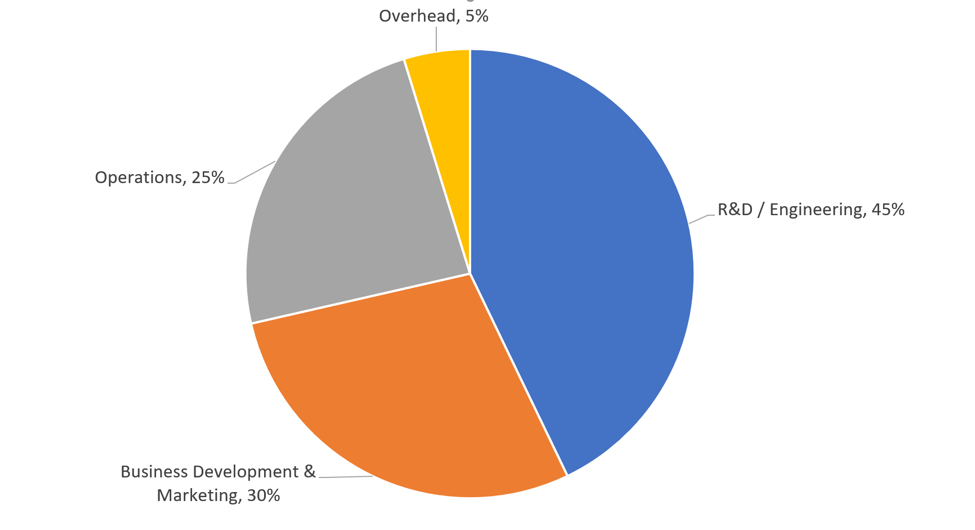
\includegraphics[width=\textwidth] {fundallocation}

\clearpage
\section {Bound Witness}
\begin{abstract}
Given that an untrusted source of data for the use of digital contract resolution (an oracle), is not useful, we can substantially increase the certainty of the data provided by first establishing the existence of a bi-directional heuristic.  The primary bi-directional heuristic is proximity since both parties can validate the occurrence and range of an interaction by cosigning the interaction.  This allows for a zero knowledge proof that the two nodes were in proximity of each other.
\end{abstract}

\subsection {Goal}
Determine the certainty that an oracle witness node in a trustless system gathered the data that it is sharing.

\subsection {Problem}
In a trustless system, a witness node can either through defect or corruption produce false data.  Invalid data can be detected and removed simply if it falls outside the allowed range for that heuristic.  Valid but incorrect data (i.e. false data) is much more difficult to detect. 

\subsection {Unidirectional vs. Bidirectional Heuristics}
Most heuristics are unidirectional, meaning that the thing being measured cannot measure back, making them very difficult to corroborate.  A bidirectional heuristic is one where the thing being measured, measures back and reports on the other party makes corroboration possible.  Location is a rare heuristic in that it can be a bidirectional with two edge nodes reporting on each other.
A real-world example of this would be if two people who are near each other take a selfie, print a copy for each party, and then both sign the selfie, giving both parties Proof of Proximity. The only way for the two to have gotten this "data" would be for them to have been together.

\subsection {Network Effect}
Imagine a system where every edge node is expected to constantly produce these "selfies" as they travel around, and store them in a binder. They are also expected to keep that binder in time order and are never allowed to delete one.  This makes a proximity recorder for the edge node that can be cross referenced with the recorders of the other edge nodes.

\subsection {Non-Edge Nodes}
All nodes are considered "witnesses", including bridges, relays, storage, and analysis nodes.  This allows for any hand-off of data to be bound.

\subsection {Cross Reference}
Analyzing every set of "selfies" that is produced and chained together by every edge node allows the system to produce the best answer of the relative proximity of all the nodes that are in the network.  If every node reports honestly and accurately, the mapping of all the relative positions of the edge nodes will achieve the maximum certainty and accuracy possible, 100 percent.  Conversely, if every node either is dishonest or flawed, the certainty and accuracy both can approach the minimum of 0 percent.

Given a set of reported data and a query for a relative position of one of the edge nodes, an approximation of the position and a certainty and accuracy coefficient can be generated.

Given the same set of data and the same analysis algorithm, every calculation should arrive at the same position approximation and certainty and accuracy coefficients.

\subsection {Diagram}
S' and S'' are each a sentinel (edge node), that collect heuristics.  When in contact with each other, they exchange heuristic data and public keys.  Both build a full record of the interaction and sign the resulting interaction.  That signed record then becomes the next entry in both of their local ledgers (16 for S' and 3 for S'').  This action binds these two witnesses as being within proximity of each other.

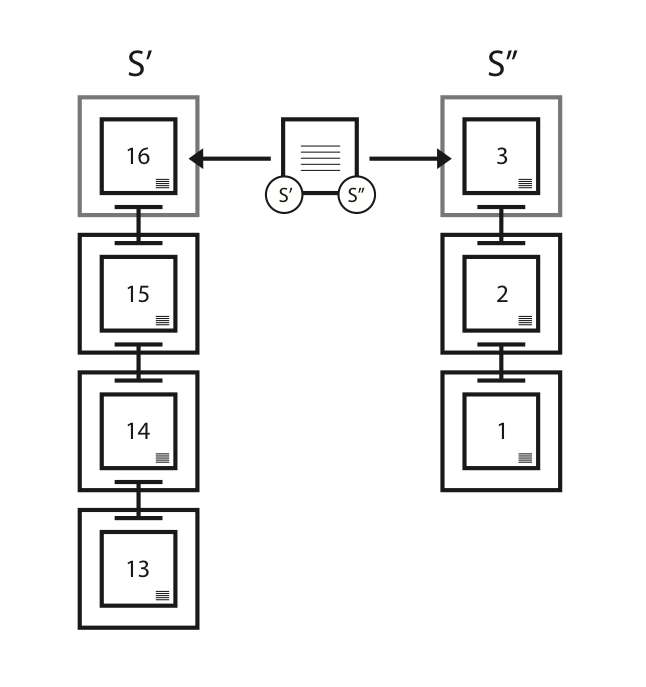
\includegraphics [width=\textwidth]{boundwitness}

\subsection {Summary}
Given a network of edge nodes that can collect signed, time sequenced, bidirectional heuristics, a relative proximity between any two of the edge nodes can be established with a high level of confidence and accuracy.

\clearpage
\section {Proof of Origin}

\begin{abstract}
With a physical network comprised of untrusted nodes it is possible to determine the certainty of data that has been provided by edge nodes based on a zero knowledge proof that two or more pieces of data originated from the same source.  Using these data sets combined with a number of similar data sets and the knowledge of at least one node's absolute location, the absolute location of the other node can be ascertained.
\end{abstract}

\subsection {Goal}
Verify that a set of heuristics come from the same origin in a trustless network.

\subsection {Problem}
In a trustless system, data may be lost, damaged, tampered with, or otherwise corrupted.  This is the core assertion of the Byzantine Generals problem.  Traditional Proof of Origin in a trustless system relies on a private key for signing transaction or contracts in a system.  This works very well with the assumption that the node on the network that signs the data in question is physically and virtually secure.  If the private key is compromised, then the ability to prove origin falters.

When applying trustless concepts to the internet of things, it must be assumed that edge nodes on the network are not physically or virtually secured, which brings forth the need to identify edge nodes without the use of IDs and to judge the data produced by them as being honest as well as valid without knowledge from outside the network. 

\subsection {Basic Functionality}
Each origin maintains its own Ledger and signs it to make a Proof of Origin Chain. Once information on the Proof of Origin Chain has been shared, it is effectively permanent, since and fork that happens after the share would end the chain and make all future data from the witness be treated as if it was from a new witness.
To generate a link in a Proof of Origin Chain, the origin generates a public/private key pair, and signs both the previous and next blocks with the same pair after including the public key in both blocks, and then immediately deletes the private key.  With the immediate deletion of the private key, the risk of a key being stolen or reused is minimized.

\subsection {Transient Key Chaining}
A series of data packets can be chained together by using temporary private keys to sign two packets in a row.  When the public key for the private key is included in the data packets, the receiver can verify that both packets were signed by the same private key.  The data in the packet cannot be altered without breaking the signature, assuring that the signed packets were not altered by a third party, such as a bridge or storage node.

\subsection {Link Depth}
At a minimum, a node generates a new public/private key pair for every link in the PoO Chain, which is a Link Depth of 1.  There may be N entries in the link table for a given Ledger Entry, with each entry specifying the distance in the future when part two of the link will be added. No two links may have the same order of magnitude on a base 2 scale. For example, [1,3,7,12,39] would be allowed, but [1,3,7,12,15] would not.

The depth 1 link is created, used and deleted when the previous block is published.  However, links of greater than depth 1 have their pair generated when the previous block is being signed, but the second signing does not happen until N locks later, after which the private key is deleted.  For this reason, links of depth greater than 1 are always considered to be less secure than links of depth 1, but they can be used to improve performance and reduce data loss at the cost of that security.

\subsection {Fixed Order}
A key method for determining the sequence of Ledgers is the order in which they were reported.  Given that it is not possible for a device to change the order of any PoO signed Ledger, when looking at all the Ledgers together, an absolute order can be established.

\subsection {Second to Last Publishing}
A primary method for establishing PoO is the fact that a Sentinel always reports their second to last block without reporting the last block.  This allows the last block to have the signed link the its predecessor as evidence of the link.

\subsection {Empty Links}
To make a PoO chain more secure, it is required that the chain is updated no more than once every ten seconds and not less than once every sixty minutes.  In the case that no new data is available, an empty block will be added to the chain.

\subsection {Diagram}
As time travels from left to right, the Proof of Origin chain that is being built gets longer.  At any given time, the producer of the chain will only provide the black border entries to a caller, waiting for the second signing of the entry before making it available.  For example, in the 3rd column, only entry 2 and 1 will be returned as being part of the chain.

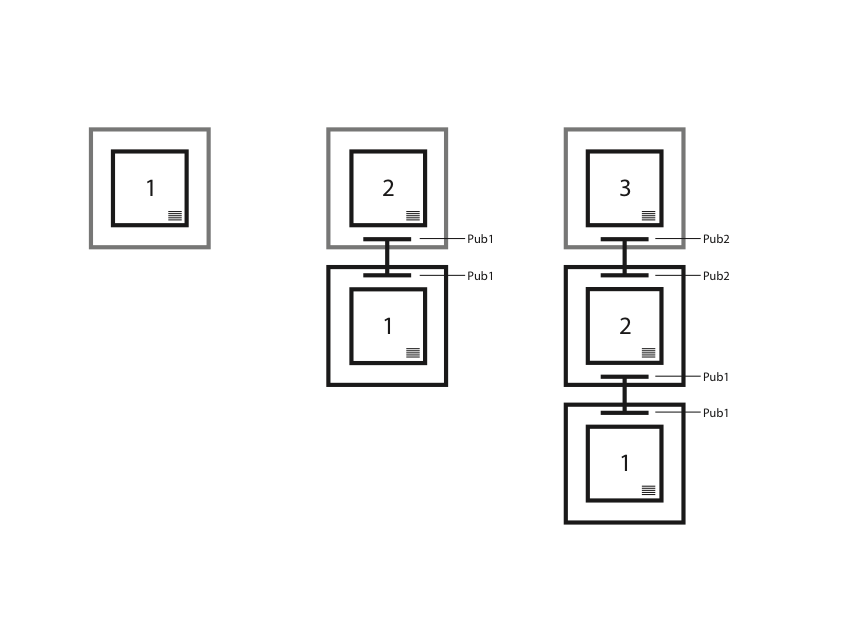
\includegraphics[width=\textwidth] {proofoforigin}

\subsection {Summary}
Given a series of data packets that are signed in sequential pairs with temporary private keys and that include the public keys, can be considered, without question, to have come from the same origin.

\clearpage
\section {Team}
XY's team is comprised of engineers, business development and marketing experts. Arie Trouw solely founded XY Findables in 2012. Scott and Markus joined as co-founders of the blockchain initiative in 2017 to assist in building the XY Oracle Network.


\begin {framed}
\begin {center}
\textbf{Arie Trouw Founder - Chief Scientist}\par
\end {center}
In 1978, at the age of 10, Arie started developing software on a TRS-80 Model I, moving on to Atari, Apple, and PC.  He also ran a series of bulletin boards centering on software and game modification.

Arie is a driven and accomplished serial entrepreneur with a rich visionary history and multiple exit events. He is a strong believer in the democratization of startup funding and creator of the integrated owner/user model. Arie began XY - The Findables Company in 2012 as Ength Degree LLC before it was converted to a C Corporation in 2016.

He currently serves as Chief Executive Officer, Chief Financial Officer, Chief Operating Officer and Chairman of the Board of Directors. Prior to starting XY-The Findables Company, Arie was CEO and Chairman of Pike Holdings Inc and Chief Technology Officer of Tight Line Technologies LLC. He received his Bachelor of Science in Computer Science from the New York Institute of Technology. Fun Fact: He is a member of one of the first Afrikaans speaking families to emigrate to the US from South Africa in 1976.
\end {framed}

\begin {framed}
\begin {center}
\textbf{Scott Scheper Co-Founder - Head of Marketing}\par
\end {center}
Since 2007, Scott has worked on many exciting ventures in the "Web 2.0" space. Some had moderate success, some failed miserably. But three have generated over 20 million in revenue each and are still actively employing people in Southern California. The first company, which is now owned by Sterkly, is where Scott met his first boss Arie Trouw. Scott joined in 2009, and over the course of a year helped grow the company to over 200 employees and generate over 80 million in revenue. The companies Scott founded are still thriving and employ a great team of software developers and other professionals in Greater San Diego, CA.

In 2013 Scott took a break from corporate life, to pursue the ideal of working remotely on a laptop while sipping tropical drinks on the powder-white beaches of St. Thomas, U.S. Virgin Islands. During this period, Scott launched Greenlamp, a programmatic advertising agency focused on direct-response marketing. The agency was built entirely using automated systems, scripts and technology with part-time software developers used sparingly to build the infrastructure. Its only full-time employee was Scott and its advertising campaigns were managed by an automated rule system, nicknamed Stewie (after the Family Guy character). Twenty-four hours a day, Stewie monitored campaigns and made automated tweaks to advertising campaigns. Stewie's feature-set even included emailing Scott to chat about the changes it made.  In its first year, Greenlamp (with Stewie's help) generated 8.59 million in revenue and still actively generates customers for clients today. 

When not crafting marketing campaigns or engrossed in the world of Ethereum, Scott can be found jogging or reading, mostly studying copywriting material written by one of his idols, Gary Halbert. When not working, he can be found spending time with friends and family in San Diego, California.
\end {framed}

\begin {framed}
\begin {center}
\textbf{Markus Levin - Co-Founder - Head of Business Development}\par
\end {center}
Markus is a seasoned "growth hacker" with 15+ years of experience in building and growing companies around the globe. After dropping out of his Phd studies at Bocconi university, he started to work with companies in the most dynamic economy in the world. During his track in the US, Markus was the CEO of ventures like Novacore, sterkly, Hive Media and Koiyo. He started to mine his first Bitcoin in 2013.
\end {framed}

\begin {framed}
\begin {center}
\textbf{Wiliam Long - Co-Founder - Head of Technology}\par
\end {center}
William is a veteran of the computer industry with over 25 years of engineering management and new product development experience.  He's also a successful entrepreneur, having founded and cofounded several computer product and data storage companies, some of which became publicly traded.  William has authored 3 US patents, and is an iOS/OSX product development authority (Apple certified developer since 1986).  He equally enjoys developing hardware and software products, and brings considerable expertise in Storage Area Networks (SANs), NAS systems, and enterprise class data storage systems for mission critical applications (such as eCommerce and medical data storage).  He received his Bachelor of Science in Electrical Engineering from Northrop University, Inglewood, CA., and is networking certified by Cisco.
\end {framed}

\begin{comment}
\section {Advisors}
The XY Oracle Network is fortunate to count a varied group of advisors to its roster of experts.

\begin {framed}
\begin {center}
\textbf{Kelsey Cole (tentative)}\par
\end {center}
Co-Founder and Chief Brand Officer at Adbank
\end {framed}

\begin {framed}
\begin {center}
\textbf{Daniel Aranda (tentative)}\par
\end {center}
Managing Director, Europe at Ripple
\end {framed}
\end{comment}

\clearpage
 
\printglossaries

\end{document}
